\section{Task: Import View Points}
\label{sec:task_import_view_points} 

This task allows importing of view points and respective ASTERIX data recording files into the opened database. It can not be run, but is performed using the GUI elements. \\

\begin{figure}[H]
  \hspace*{-2.5cm}
    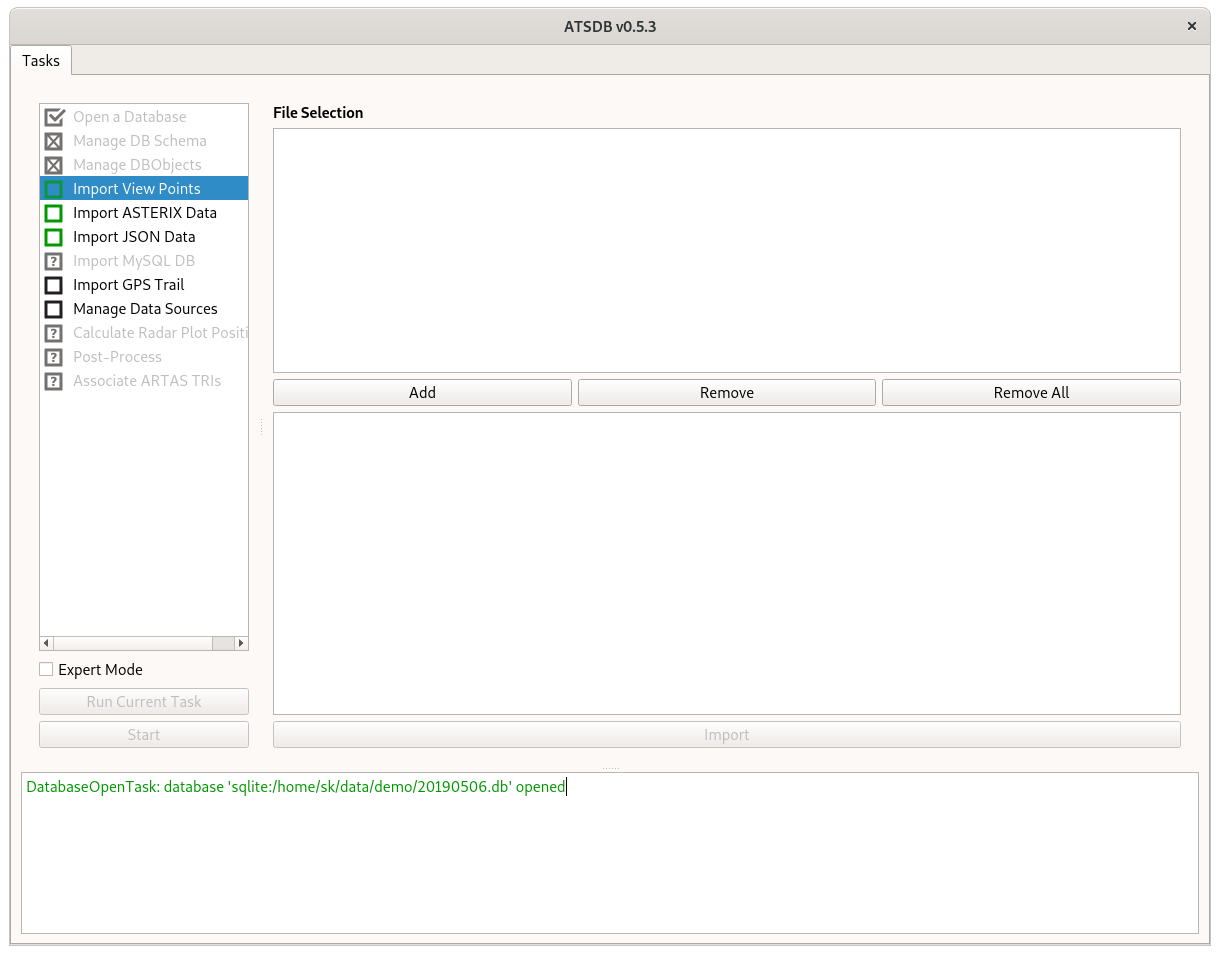
\includegraphics[width=19cm]{figures/view_point_import_task.png}
  \caption{Task: Import View Points}
\end{figure}

In the 'File Selection' list, a list of available view point JSON files is given. Entries can be added using the 'Add' button or removed using either the 'Remove' or 'Remove All' buttons. \\

Below a text field is given which, after selection of a view point file, displays the view point context information or an error message. \\

At the bottom, an 'Import' button exist, which is only enabled if a valid file was selected.

\subsection{Notes}

For a detailed specification of a view point file, please refer to \nameref{sec:appendix_view_points}. \\

For each of the datasets, an 'Import ASTERIX Data' task is started, in the configuration that was set previously. Please make sure that the configuration is valid for such processing. \\

For the filename in each dataset, the absolute path is searched first. If such a file can not be found, a file with the same name but in the location of the view point file is searched also. If the referred file can not be found, an error message is displayed. \\

It is not recommended to import multiple view point files, such a use case is not yet fully supported.

\subsection{Importing}

Please add and select the file to be imported, after which the 'Import' button will become available. \\

\begin{figure}[H]
    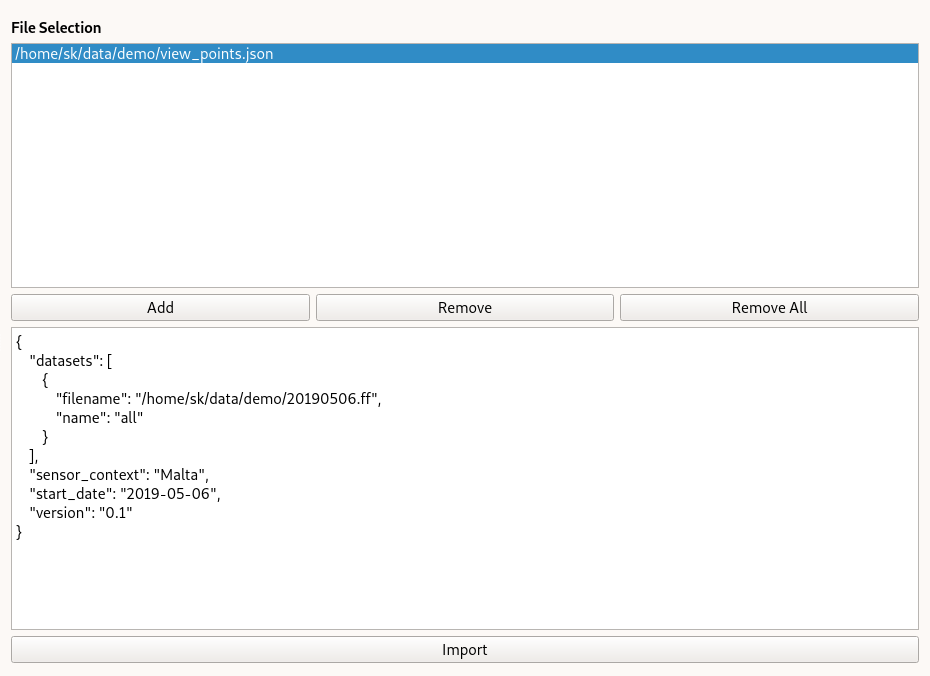
\includegraphics[width=16cm,frame]{figures/view_point_import_ready.png}
  \caption{Task: Import View Points Ready}
\end{figure}

In the shown example, one dataset is specified. Please click 'Import' to start the view points and ASTERIX data import. \\

After a successful import the information is logged and the next recommended task is available.

